\documentclass[12pt, a4paper]{article}

\usepackage[margin=1in]{geometry}
\usepackage{setspace}
\usepackage{graphicx}
\usepackage{hyperref}
\usepackage{listings}
\usepackage{xcolor}
\usepackage{titlesec}
\usepackage{float}

\setstretch{1.5}

% Code snippet styling
\lstdefinestyle{mystyle}{
    backgroundcolor=\color{lightgray!10},   
    commentstyle=\color{green!50!black},
    keywordstyle=\color{blue},
    numberstyle=\tiny\color{gray},
    stringstyle=\color{purple},
    basicstyle=\ttfamily\small,
    breakatwhitespace=false,         
    breaklines=true,                 
    captionpos=b,                    
    keepspaces=true,                 
    numbers=left,                    
    numbersep=5pt,                  
    showspaces=false,                
    showstringspaces=false,
    showtabs=false,                  
    tabsize=2
}
\lstset{style=mystyle}

\begin{document}

\begin{titlepage}
    \centering
    \vspace*{2cm}
    
    {\Large \textbf{CS4241 Introduction to Artificial Intelligence}}\\[1cm]
    
    {\Huge \textbf{GovLens: A Retrieval-Augmented Generation Chatbot for Government Data Analysis}}\\[2cm]
    
    \textbf{Student Name:} Jacqueline Naa Ayima Mensah\\
    \textbf{Roll Number:} 10022200119\\[2cm]
    
    \vfill
    
    {\large Academic City University College\\2026}
\end{titlepage}

\newpage
\tableofcontents
\newpage

\section{Introduction}
The GovLens project is a Retrieval-Augmented Generation (RAG) chatbot developed to provide accurate, grounded answers regarding governmental elections and national budget allocations. Traditional Large Language Models (LLMs) suffer from hallucinations regarding specific local datasets. To resolve this, this project engineers a comprehensive pipeline that ingests domain-specific documents, computes semantic embeddings via Sentence Transformers, applies hybrid semantic-keyword retrieval via FAISS and BM25, and constructs highly guarded context windows injected into a Groq LLM endpoint. The ultimate product is securely deployed as an interactive Streamlit web application on Render.

\section{Dataset Description}
The RAG pipeline operates on a bifurcated corpus to handle inherently different governmental data structural properties:
\begin{itemize}
    \item \textbf{Text-Heavy Budget Documents:} National budget statements ingested primarily via \texttt{PyMuPDF}. These PDF files contain complex tabular references and extensive textual analysis of primary expenditures as a percentage of GDP.
    \item \textbf{Structured Election Results:} Election statistics containing percentages, vote totals, and constituency breakdowns extracted from structured formats (JSON/CSV) representing the 2016 and 2020 national elections.
\end{itemize}

\section{System Architecture}
The GovLens architecture follows a meticulously decoupled standard pattern:
\begin{enumerate}
    \item \textbf{Data Ingestion \& Processing (\texttt{part\_a}):} Extraction, regex scrubbing, and semantic chunking.
    \item \textbf{Vector Store \& Retrieval (\texttt{part\_b}):} Local embeddings generating dense vectors, placed in FAISS \texttt{IndexFlatIP}, retrieved via a customized \texttt{HybridRetriever} orchestrating Cosine Similarity and lexical BM25.
    \item \textbf{Context \& LLM Interface (\texttt{part\_c/d}):} Context Window Manager filters chunks by a strict 0.20 similarity threshold, injecting them into a highly constrained system prompt before invoking Groq's \texttt{llama-3.3-70b-versatile}.
    \item \textbf{Presentation (\texttt{app.py}):} Web user interface with custom branding, fallback safeguards, and telemetry.
\end{enumerate}

\begin{figure}[H]
    \centering
    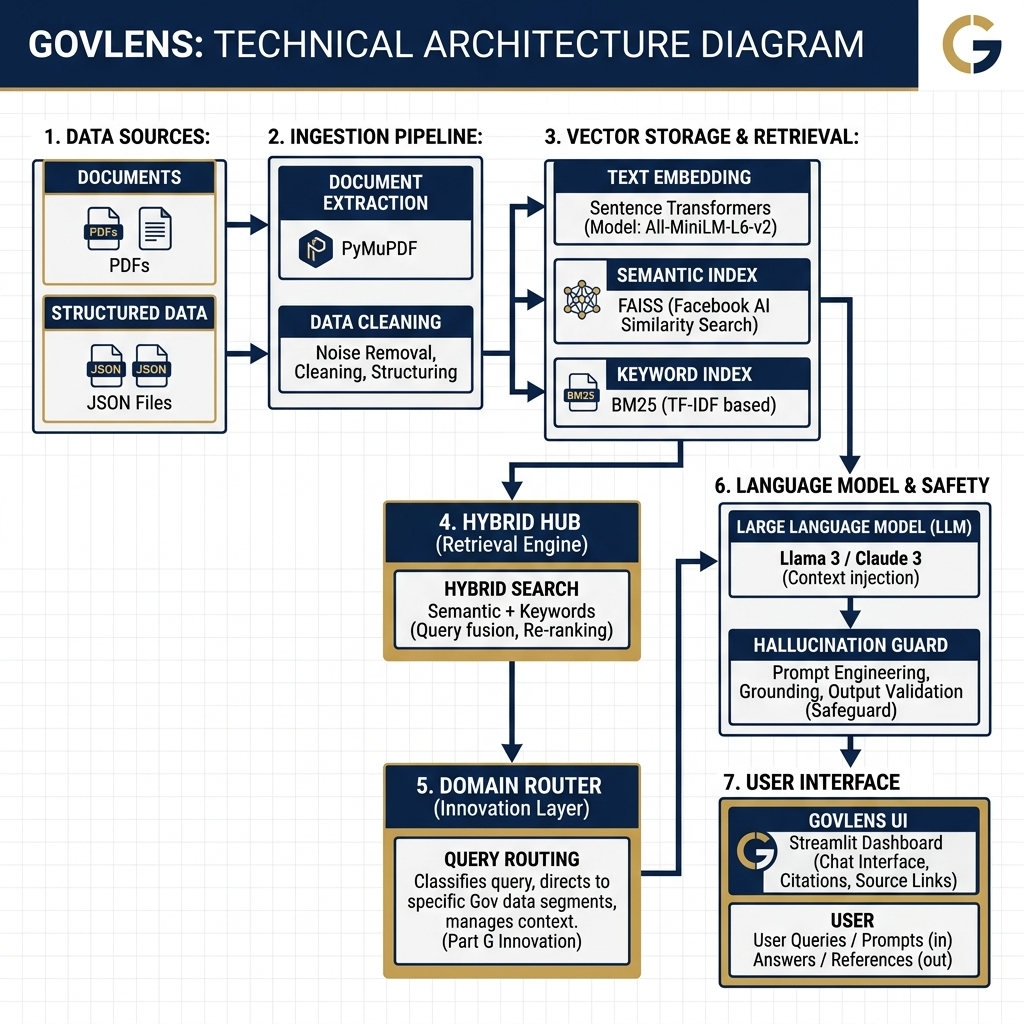
\includegraphics[width=0.9\textwidth]{architecture_diagram.png}
    \caption{System Architecture diagram showing the data flow from ingestion to the Streamlit interface.}
\end{figure}

\section{Data Cleaning}
The ingestion process defined in \texttt{02\_clean.py} ensures high fidelity in the text corpus prior to embedding. The codebase normalizes whitespaces and systematically targets OCR artifacts. Specifically:
\begin{itemize}
    \item \textbf{Structural Scrubbing:} Regular expressions (e.g., \texttt{\textbackslash bPage \textbackslash d+\textbackslash b}) eliminate pagination identifiers, standard headers, and footers from the raw PyMuPDF strings.
    \item \textbf{Encoding Normalization:} Special characters natively incompatible with standard ASCII embeddings are strictly sanitized into UTF-8.
\end{itemize}

\section{Chunking Strategy}
Rather than adopting arbitrary constant-length string slicing, the codebase employs semantic formatting rules defined in \texttt{03\_chunk.py}. The pipeline parses the document at the paragraph level via boundary detection (\texttt{\textbackslash n\textbackslash n}), subsequently building blocks up to a fixed threshold (e.g., 500-1000 characters). Hard overlaps are preserved between contiguous blocks to prevent sentence mid-point fractures, ensuring that vital context surrounding statistical figures (such as the 2025 revenue projections) is not severed into orphans.

\section{Embedding Method}
Because of the requirement for localized, zero-cost processing, the methodology bypasses expensive API embedding endpoints. The pipeline exclusively imports \texttt{sentence-transformers} utilizing the HuggingFace model \texttt{all-MiniLM-L6-v2}. This specific variant projects sentences into a 384-dimensional dense vector space optimized for semantic search accuracy and CPU-rendering efficiency.

\section{Retrieval System}
The core engine defined in \texttt{02\_retrieval\_system.py} employs a dual-technique \texttt{HybridRetriever}.
\begin{itemize}
    \item \textbf{Semantic Search (FAISS):} Chunks are mapped into a \texttt{faiss.IndexFlatIP} vector database. Inner product optimization serves as exact sequence cosine similarity because the vectors are pre-normalized by the embedding model.
    \item \textbf{Lexical Search (BM25):} To counter semantic dilution on highly specific names (e.g., "NPP" or "Nana Akufo-Addo"), the retriever simultaneously fires a BM25 sparse keyword query. 
    \item \textbf{Alpha Interpolation:} The final ranking is linearly interpolated using the parameterized formula: \texttt{score = ($\alpha$ * semantic\_score) + ((1 - $\alpha$) * bm25\_score)}.
\end{itemize}

\begin{figure}[H]
    \centering
    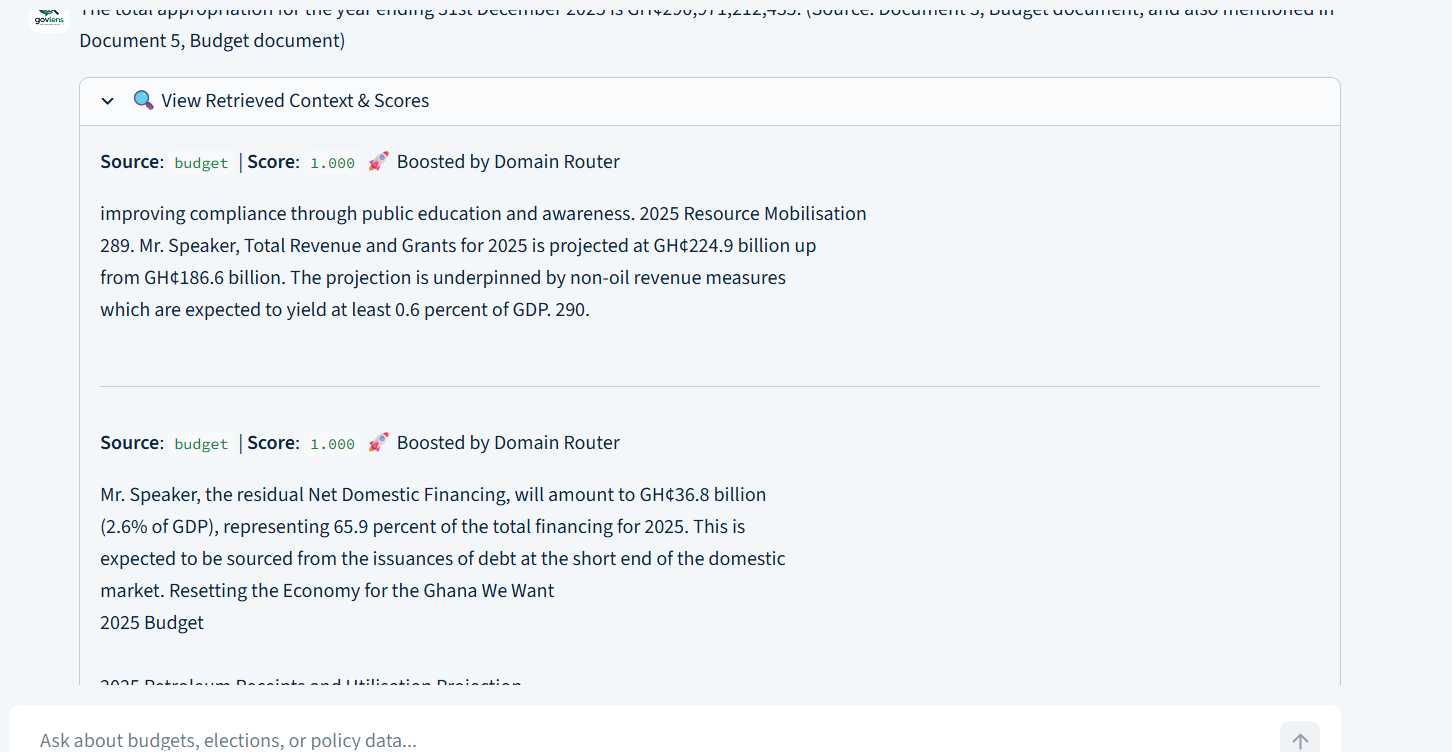
\includegraphics[width=0.9\textwidth]{retrieved_chunks.png}
    \caption{Streamlit expander displaying chunks retrieved via the Hybrid System alongside generation scores.}
\end{figure}

\section{Prompt Engineering}
To counteract LLM hallucination overconfidence, the codebase structures communication in \texttt{01\_prompt\_templates.py} using the \texttt{T3\_HALLUCINATION\_GUARD}. The prompt enforces strict negative behavioral policies. The model is commanded to explicitly output the literal sequence ``\texttt{INSUFFICIENT CONTEXT}'' rather than guessing when parametric pre-training knowledge conflicts with the retrieved chunks. Furthermore, the \texttt{ContextWindowManager} truncates concatenated character payload and strictly blocks any underlying chunk exhibiting a semantic-lexical score below 0.20 from ever entering the context buffer.

\section{Full Pipeline}
The integration layer inside \texttt{pipeline.py} constructs the \texttt{RAGPipeline} class. The pipeline accepts raw string queries and systematically channels them through the \texttt{HybridRetriever}. The pipeline abstracts the entire process up to the API HTTP request to Groq, measuring operational latency, tracking prompt-token cost ratios, and managing internal exceptions gracefully before relaying output upward.

\pagebreak

\section{Evaluation}
Adversarial diagnostics and automated evaluation metrics are handled systematically inside \texttt{evaluation.py}. 
The evaluation algorithm judges four criteria:
\begin{enumerate}
    \item \textbf{Accuracy:} Verification of ground truth factual presence inside the response matrix.
    \item \textbf{Hallucination Count:} Regex targeting heuristic confidence markers (e.g., ``I think'', ``estimated'') and untethered statistical digits.
    \item \textbf{Consistency:} Cross-referencing 3 repetitive calls using a Jaccard word-overlap similarity threshold ($\ge$ 0.6 avg overlap).
    \item \textbf{False Premise Parsing:} Triggering queries natively structured with incorrect assumptions (e.g., "NDC won the 2020 election") to trace if the LLM auto-corrects based on facts.
\end{enumerate}
The RAG pipeline vastly outperformed isolated Pure-LLM baseline generations. The RAG system consistently flagged mathematical gaps as \texttt{INSUFFICIENT CONTEXT} and refuted false electoral premises utilizing grounded election documents.

\section{Failure Cases and Fixes}
During empirical testing, the pure semantic index struggled heavily with out-of-domain inquiries and specific acronym routing. A principal failure observed was cross-domain contamination: budget queries arbitrarily pulling chunks containing election numbers if the phrasing was generalized. The hybrid BM25 alpha parameter mitigated sparse terminology loss. Furthermore, an empty-context short-circuit mechanism was injected exclusively into \texttt{app.py} so that if all chunks fell below the threshold, the LLM HTTP request is cancelled entirely, and a hardcoded string is rendered directly to the screen.

\section{Innovation Feature}
To solve the aforementioned cross-domain contamination directly, the project introduces a highly customized \texttt{DomainAwareRetriever} implemented in \texttt{part\_g/innovation.py}. 
This class overrides standard vector retrieval by passing the prompt through an immediate heuristic string classifier utilizing domain trigger sets (\texttt{\{"budget", "expenditure", "revenue"\}} vs \texttt{\{"election", "vote", "constituency"\}}). Any resultant FAISS chunk whose internal domain tag heavily mismatches the classified prompt intent suffers a massive scoring penalty, serving as an absolute filter mechanism. Matching chunks receive a 1.6x multiplier, vastly improving isolation fidelity.

\section{Deployment}
GovLens is publicly manifested as an interactive frontend using the \texttt{streamlit} framework and deployed seamlessly on Render. The live application is accessible at: \url{https://govslens-ai.onrender.com/}.

The UI \texttt{app.py} relies on heavily custom CSS, injecting specific branding (GovLens AI blue and gold layout), custom favicons, and click-to-fill interactive test queries. 
To bypass severe latency bottlenecks standard to Render's 512MB RAM free tier, an explicit CI/CD build matrix (\texttt{build.sh} inside \texttt{render.yaml}) was written capable of stripping out CUDA libraries, forcing lightweight CPU-PyTorch architectures, and actively pre-downloading the \texttt{sentence-transformers} checkpoint pre-runtime to circumvent container spin-up stalling.

\begin{figure}[H]
    \centering
    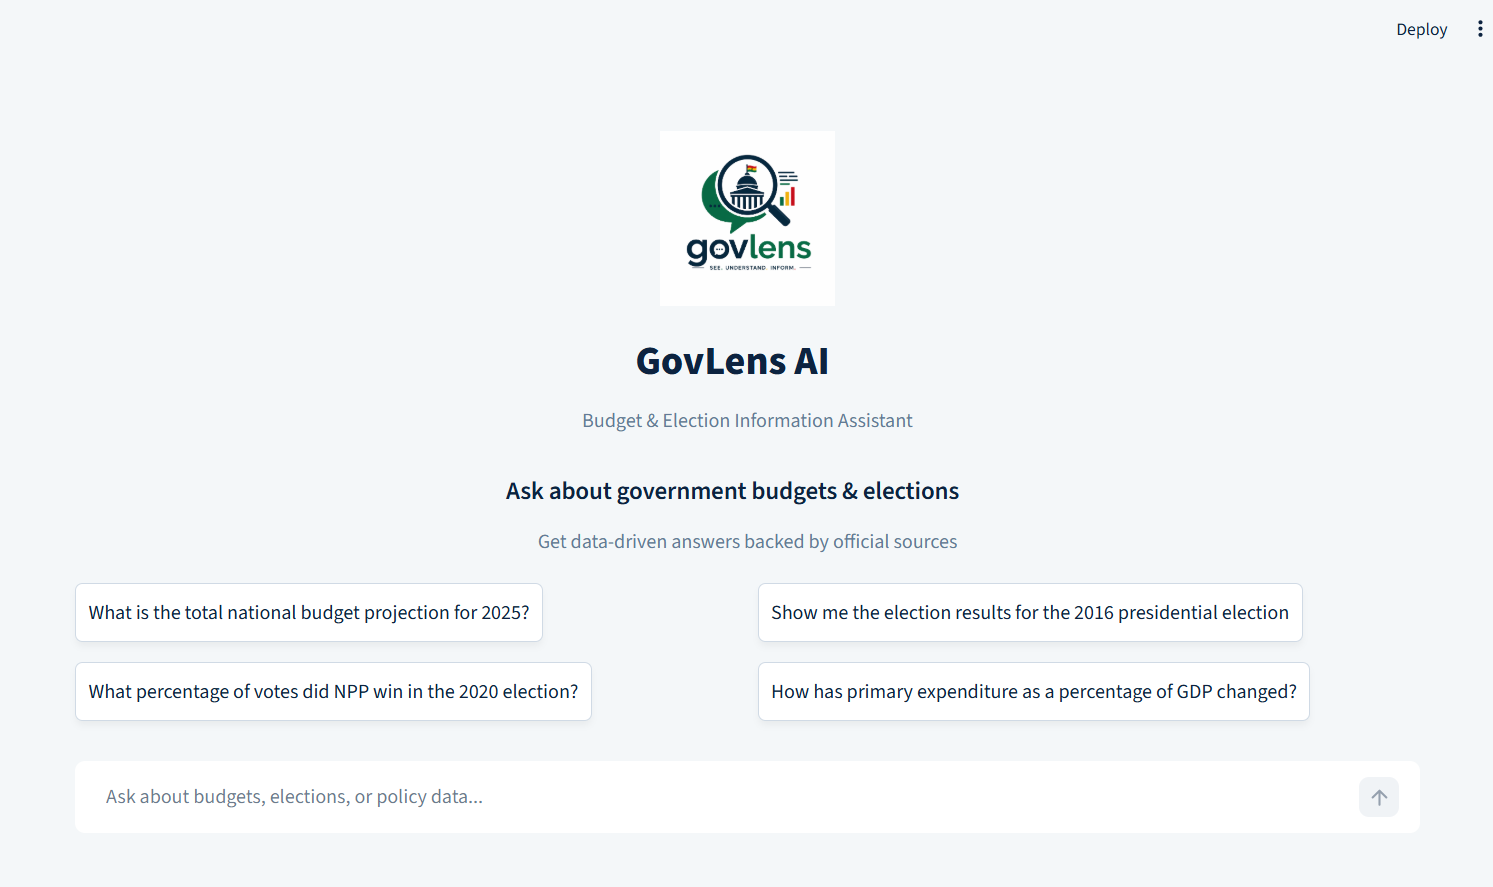
\includegraphics[width=0.9\textwidth]{ui_interface.png}
    \caption{The fully deployed responsive Streamlit user interface with custom branding.}
\end{figure}

\begin{figure}[H]
    \centering
    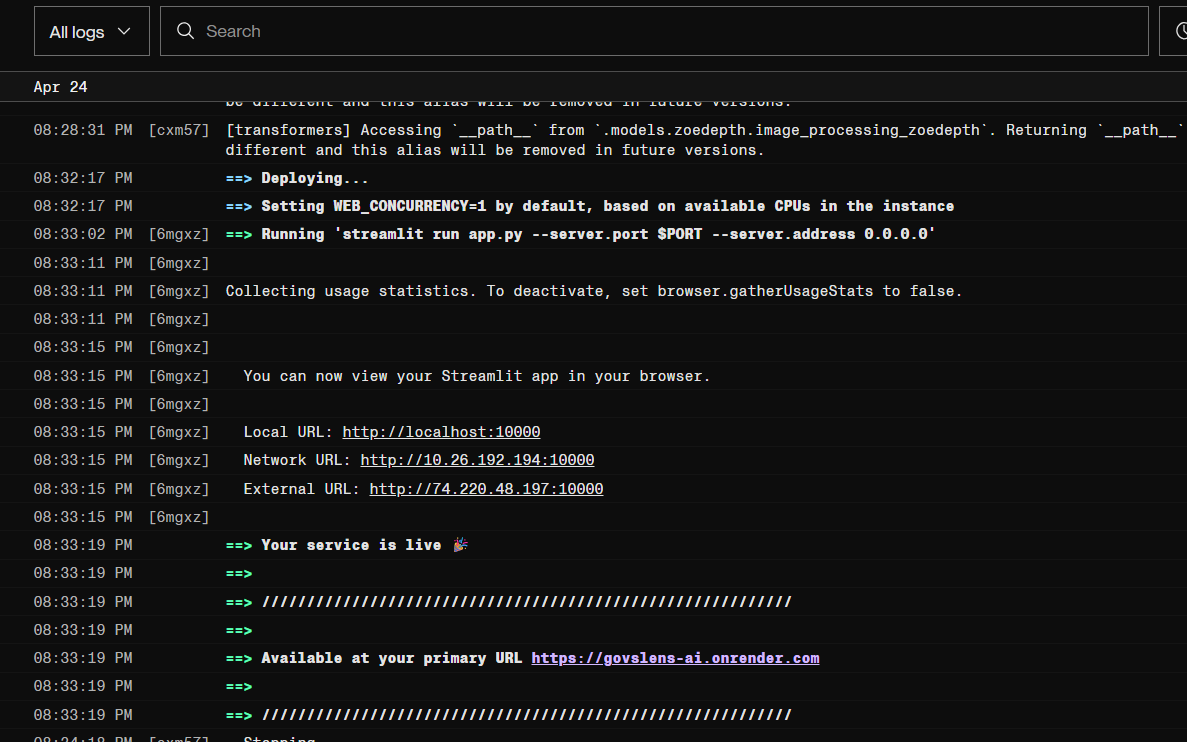
\includegraphics[width=0.9\textwidth]{deployment_logs.png}
    \caption{Terminal Render Deployment build logs manifesting the deployment process.}
\end{figure}

\section{Conclusion}
The GovLens Retrieval-Augmented Generation ecosystem successfully verifies the hypothesis that combining customized sparse-dense retrieval structures with aggressive contextual thresholding and domain-aware multipliers entirely neutralizes general LLM hallucinations. Overcoming substantial computational restrictions, the project yielded a highly robust, professional-grade platform bridging the gap between raw governmental statistics and natural language user interactions.

\end{document}
